\documentclass[12pt,oneside]{book}
\usepackage{fullpage}
\usepackage{color}
\usepackage{mathtools}
\usepackage{amsmath}
\usepackage{amsfonts}
\usepackage{graphicx}
\usepackage{lipsum}
\usepackage[utf8]{inputenc}
\usepackage{geometry}
%%\graphicspath{ {~/Desktop/thesis/thesis/} }

\geometry{
 a4paper,
 total={210mm,297mm},
 left=35mm,
 right=25mm,
 top=25mm,
 bottom=25mm,
}

\newif\ifquoteopen
\catcode`\"=\active % lets you define `"` as a macro
\DeclareRobustCommand*{"}{%
   \ifquoteopen
     \quoteopenfalse ''%
   \else
     \quoteopentrue ``%
   \fi
}

%Gummi|065|=)

\date{}
\begin{document}

%% ----------------------------------------------PAGE 1 TITLE

\begin{titlepage}
    \begin{center}
        \vspace*{1cm}
        
        {\scshape {\huge{I}\Large{NTER-PROCEDURAL} \huge{A}\Large{NALYSIS OF}\\
                   \vspace{0.1cm}
				   \huge{C}\Large{ONCOLIC } \huge{E}\Large{XECUTION}}}\\[2.0cm] % Thesis title

        
        \textit{A Thesis Submitted\\
        in Partial Fulfilment of the Requirements\\
        for the Degree of\\}
                \vspace{0.8cm}
        \textbf{\large{MASTER OF TECHNOLOGY}}\\[0.5\baselineskip]
        \textit{by}\\[0.5\baselineskip]
        \textbf{\large{Ashwini Kshitij}}\\
                \vspace{0.8cm}
        \textit{supervised by}\\
                \vspace{0.8cm}
        \textbf{\large{Dr. Subhajit Roy}}\\
        \textbf{\large{Dr. Amey Karkare}}
        \vspace{0.8cm}
        
      	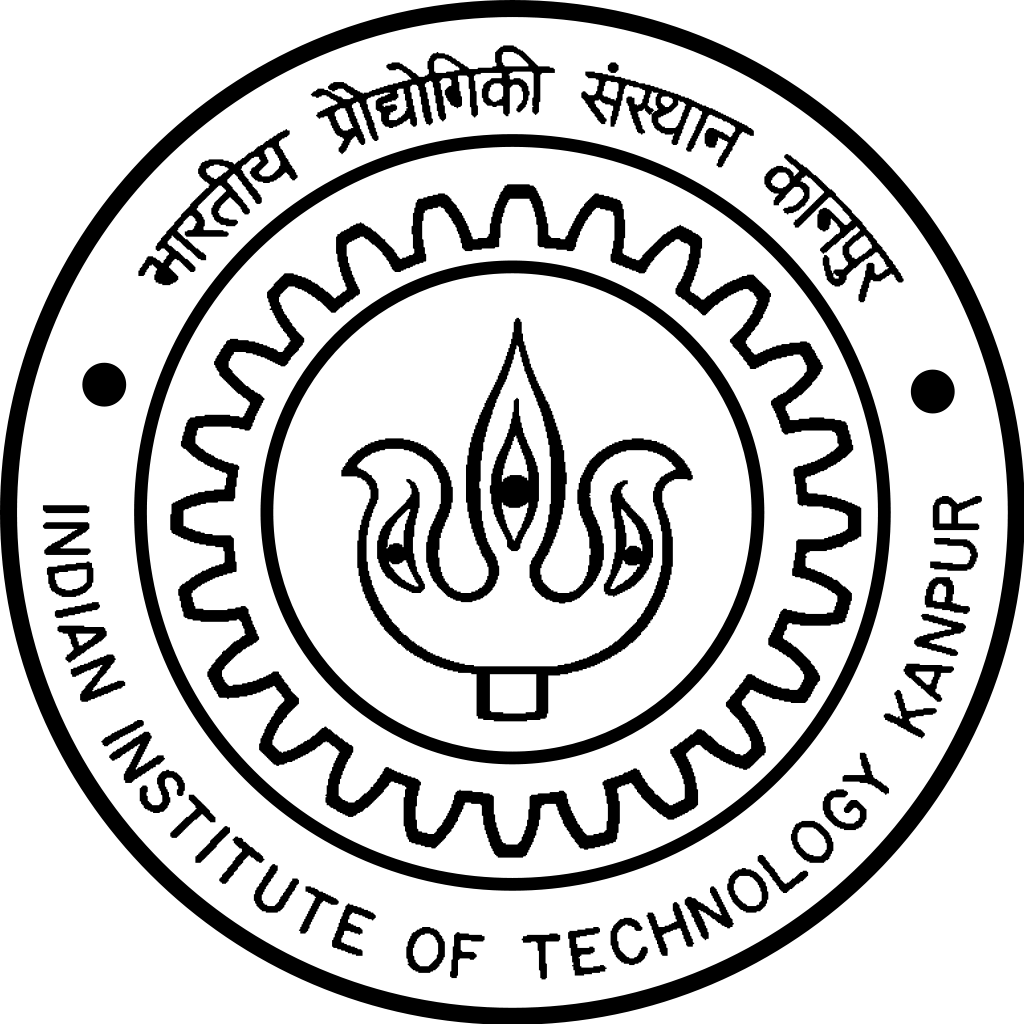
\includegraphics[width=0.25\textwidth]{iitklogo.png}
        
        \vspace{1\baselineskip}
        
        \uppercase{Department of Computer Science and Engineering\\
        \textbf{Indian Institute of Technology Kanpur}}\\
        
        \vspace{1\baselineskip}
        \textbf{June 2015}
        
    \end{center}
\end{titlepage}


%%-----------------------------------------------PAGE 2 Certificate

\frontmatter
\addcontentsline{toc}{chapter}{Certificate}
\begin{center}
\textbf{\Large{CERTIFICATE}}
\end{center}
\vspace*{3\baselineskip}
This is to certify that the work contained in this thesis entitled \textbf{\textit{"Inter-procedural analysis of Concolic Execution"}}, by \textbf{Ashwini Kshitij (Roll No. 10327165)}, has been carried out under my supervision and this work has not been submitted elsewhere for a degree.\\
\\[4\baselineskip]

  \small
  \vspace{2.0 cm}
  \begin{tabular*}{1.0\textwidth}{@{\extracolsep{\fill}} l r}
    \textbf{Dr. Subhajit Roy} 			 & 				\textbf{Dr. Amey Karkare}\\
    Assistant Professor,				 &				Assistant Professor,\\
    Department of CSE, 					 & 				Department of CSE,\\
    IIT Kanpur.							 &				IIT Kanpur.
    
  \end{tabular*}
\newpage


%%----------------------------------------------ABSTRACT
\addcontentsline{toc}{chapter}{Abstract}
\begin{center}
\textbf{\Large{ABSTRACT}}
\end{center}

Still have to think of something.


\newpage

%%----------------------------------------------ACKNOWLEDGMENT
\addcontentsline{toc}{chapter}{Acknowledgement}
\begin{center}
\textbf{\Large{Acknowledgements}}
\end{center}

\vspace{1.0 cm}

I acknowledge, with gratitude, my debt of thanks to Professor Subhajit Roy for his advise and encouragement and to Professor Amey Karkare for his aid and foresight. They presented me with the opportunity to tackle interesting problems in field of Software Testing. Their patient but firm guidance was critical to successful completion of my research.  

\vspace{0.5 cm}

I appreciate the support of my friends and wingmates (except one) who always provided me with the confidence and courage to tackle even the most challenging problems. Without their help and councel, the completion this work would have been immeasurably more difficult. 

\vspace{1.0 cm}

I also want to express my sincere gratitude to \textit {\textbf {BRNS}} for encouraging our research work. Their unshaken faith in our efforts motivated me to follow through this project.

\begin{flushright}
\textbf{-Ashwini Kshitij}
\end{flushright}

\newpage

%%----------------------------------------------CONTENTS

\tableofcontents
\mainmatter

%%---------------------------------------------CHAP 1 Intro

\chapter{Introduction}

This is where we write.



\end{document}
